%(BEGIN_QUESTION)
% Copyright 2006, Tony R. Kuphaldt, released under the Creative Commons Attribution License (v 1.0)
% This means you may do almost anything with this work of mine, so long as you give me proper credit

Noen prosesser kan reguleres med en automatisk regulator som kun har {\it integralvirkning}. Her er et skjemadiagram for en slik regulator:

$$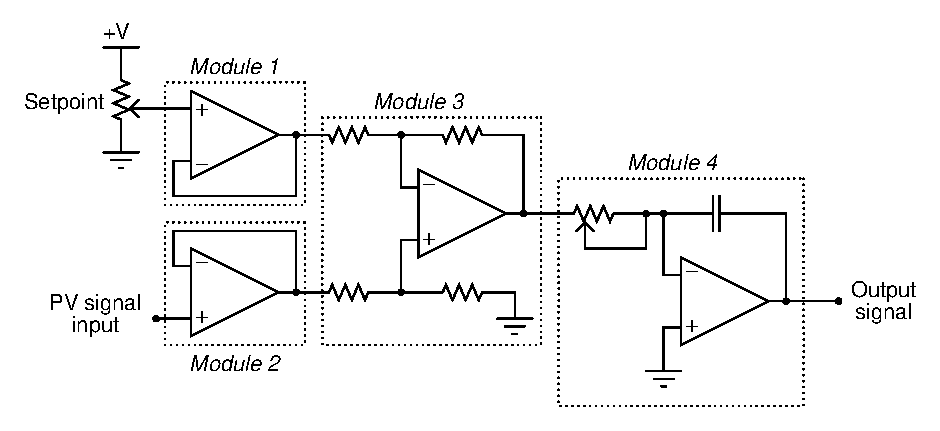
\includegraphics[width=15.5cm]{i01588x01.eps}$$

Studer skjemadiagrammet og svar deretter på følgende spørsmål:

\begin{itemize}
\item{} Vis hvor ``avvik'' beregnes i kretsen
\item{} Bestem om dette er en direktevirkende eller reversvirkende regulator
\item{} Identifiser hvordan man kan {\it redusere} integrasjonstidskonstanten ($\tau_i$), dvs. hvordan man kan {\it øke} aggressiviteten i integralvirkningen
\end{itemize}

\vskip 20pt \vbox{\hrule \hbox{\strut \vrule{} {\bf Forslag til sokratisk diskusjon} \vrule} \hrule}

\begin{itemize}
\item{} Hvis denne brukes til å regulere en virkelig prosess, vil regulatoren få {\it offset} slik en regulator med bare proporsjonalvirkning får? Forklar hvorfor eller hvorfor ikke.
\item{} Beskriv virkningen dersom tilbakekoblingsledningen i modul 2 feiler åpen.
\item{} Beskriv virkningen dersom den nedre venstre motstanden i modul 3 feiler åpen.
\item{} Beskriv virkningen dersom den øvre venstre motstanden i modul 3 feiler åpen.
\item{} Beskriv virkningen dersom den nedre høyre motstanden i modul 3 feiler åpen.
\item{} Beskriv virkningen dersom den øvre høyre motstanden i modul 3 feiler åpen.
\item{} Beskriv virkningen dersom kondensatoren i modul 4 feiler kortsluttet.
\end{itemize}

\underbar{file i01588}
%(END_QUESTION)





%(BEGIN_ANSWER)

\begin{itemize}
\item{} Vis hvor ``avvik'' beregnes i kretsen: {\bf Ved utgangen av differensialforsterkeren (modul 3)}
\item{} Bestem om dette er en direktevirkende eller reversvirkende regulator: {\bf Reversvirkende}
\item{} Identifiser hvordan man kan {\it redusere} integrasjonstidskonstanten ($\tau_i$), dvs. hvordan man kan {\it øke} aggressiviteten i integralvirkningen: {\bf Mindre kondensator i modul 4, lavere potmeterinnstilling i modul 4, økt differensiell spenningsforsterkning i modul 3}
\end{itemize}

%(END_ANSWER)





%(BEGIN_NOTES)


%INDEX% Control, integral: analog electronic controller

%(END_NOTES)
